\titleformat{\chapter}[display]
{\normalfont\huge\bfseries}{Capítulo \thechapter}{0.5em}{\huge}
\titlespacing*{\chapter}{0pt}{-1.25cm}{25pt}
\chapter{Introducción}
\section{Concepto de arritmia}
Las enfermedades cardiovasculares son la primera causa de muerte en el mundo \cite{roth2020global} y una de las causas más comunes de estas enfermedades son las arritmias.

Una arritmia cardiaca es un resultado de una alteración en la iniciación o propagación del ritmo del corazón \cite{velez}. Si se produce una arritmia, el corazón puede tener un ritmo demasiado rápido, demasiado lento o irregular. Esto puede provocar síntomas como palpitaciones, mareos, falta de aire e incluso desmayos, y estas pueden llegar a ser mortales.

Los cardiólogos utilizan dispositivos como un \textit{Holter}\footnote{\textbf{Holter}: Dispositivo médico portátil que se utiliza para monitorear y registrar la actividad eléctrica del corazón durante un período prolongado} para generar electrocardiogramas (ECG), que son diagramas que representan los latidos del corazón y con ellos son capaces de analizarlos y encontrar anomalías cardiacas.

Entre esas anomalías están las contracciones prematuras del corazón, un tipo de arritmia que este proyecto se encargará de detectar. 

\begin{figure}[h!]
	\centering
	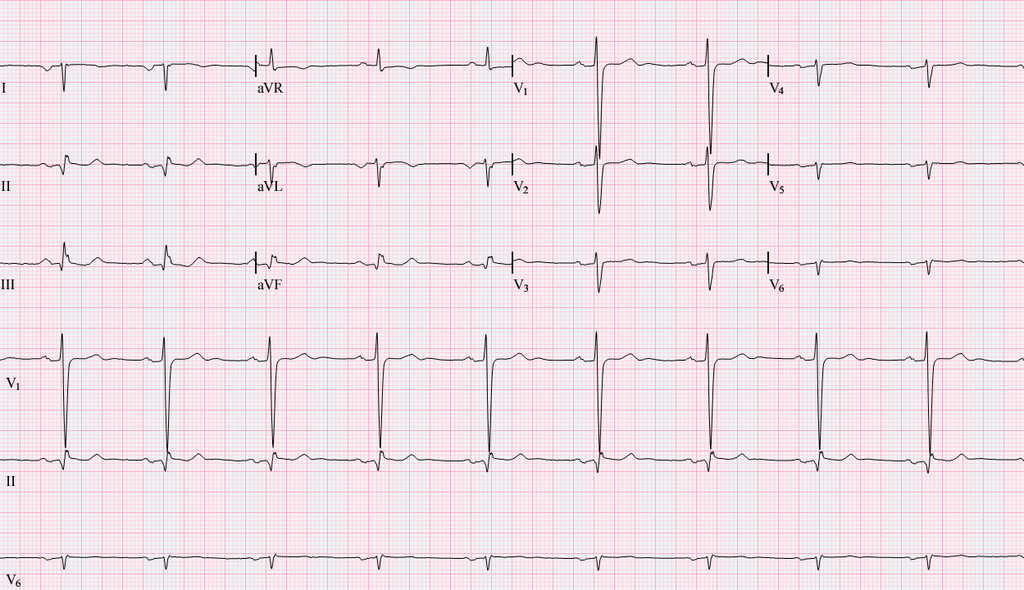
\includegraphics[width=0.7\textwidth]{./Images/img_introduccion/electrocardiograma.png}
	\caption{Imagen de varios electrocardiogramas recopilados por un \textit{Holter} \cite{fotoElectrocardiograma}}.
	\label{fig:electrocardiogramas}
\end{figure}

\section{Algoritmo de detección}
El algoritmo de detección de arritmias que sigue este proyecto se basa en la detección de 
los picos QRS producidos en el electrocardiograma.

Un pico QRS, como se muestra en la \Cref{fig:complejoQRS}, en un electrocardiograma es causado por la contracción del ventrículo al bombear la sangre por las arterias. Este es el impulso eléctrico más fuerte que el corazón produce en cada latido \cite{wiki:QRS_complex}. En este proyecto utilizaremos estos picos para comparar la distancia entre ellos y poder determinar si se ha producido una arritmia. 

\begin{figure}[h]
	\centering
	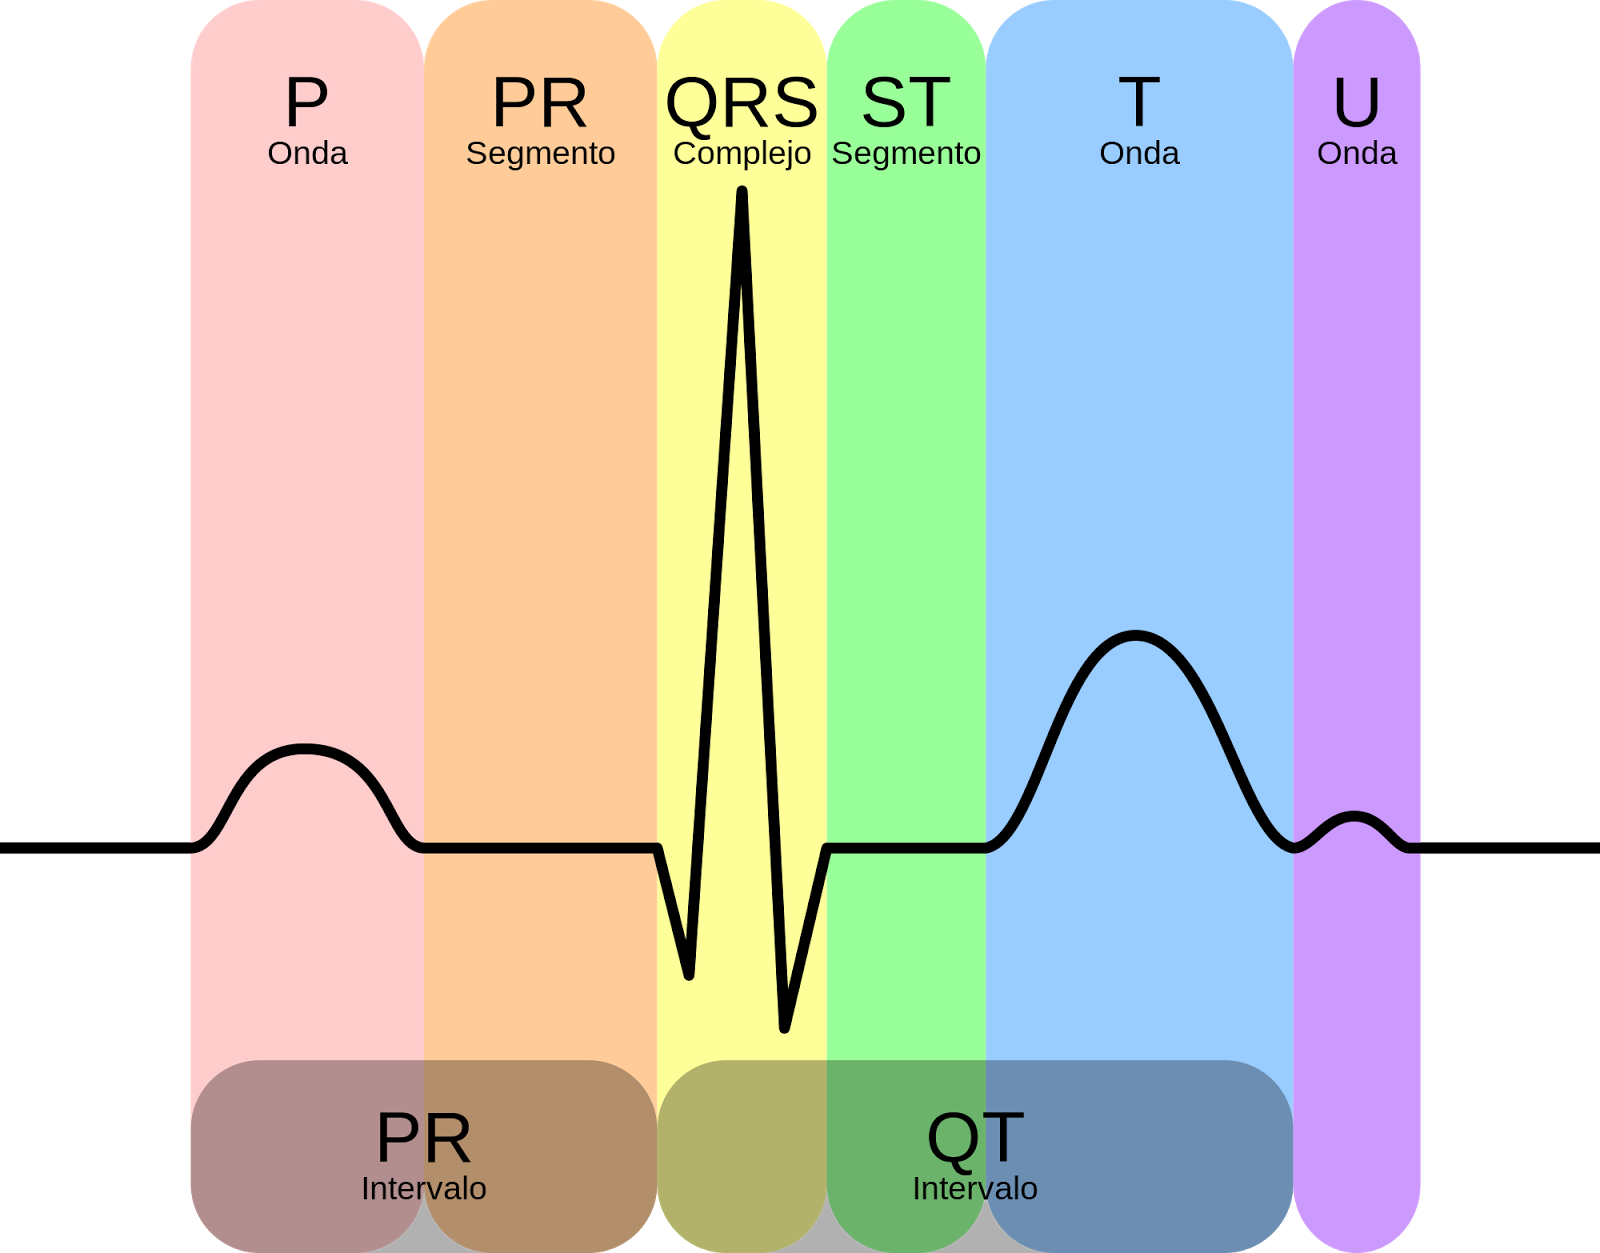
\includegraphics[width=0.4\textwidth]{./Images/img_introduccion/complejoQRS.png}
	\caption[Complejo QRS]{Complejo QRS \cite{desai2021low}}
	\label{fig:complejoQRS}
\end{figure}

Este algoritmo es de especial interés\cite{kiranyaz2011personalized}, ya que el desarrollo de técnicas eficientes para automatizar el análisis de ECG es fundamental para ayudar a los cardiólogos en sus diagnósticos, especialmente en la detección de arritmias. El cardiólogo tendría que dedicar varios minutos para hallar arritmias en un electrocardiograma de, por ejemplo, 30 minutos. Este algoritmo no pretende ser una solución definitiva para la detección de arritmias, ya que se requieren varios años de estudio para entenderlas completamente. Por ello, se enfoca en detectar contracciones ventriculares prematuras.

\subsection{Filtrado}
Como se puede observar en la \Cref{fig:102filtradoysinfiltrar} es conveniente hacer un filtrado de las tiras de ritmo para poder detectar mejor los picos QRS, ya que el filtrado centra la onda de la señal en el valor 0 y evita fallos en el algoritmo de detección de picos del que se hablará más adelante. 

En la creación del proyecto se ha intentado no filtrar la onda para comprobar si se obtienen mejores resultados que sin dicho filtrado, pero no se ha dado el caso por las irregularidades de la misma.

\begin{figure}[h!]
	\centering
	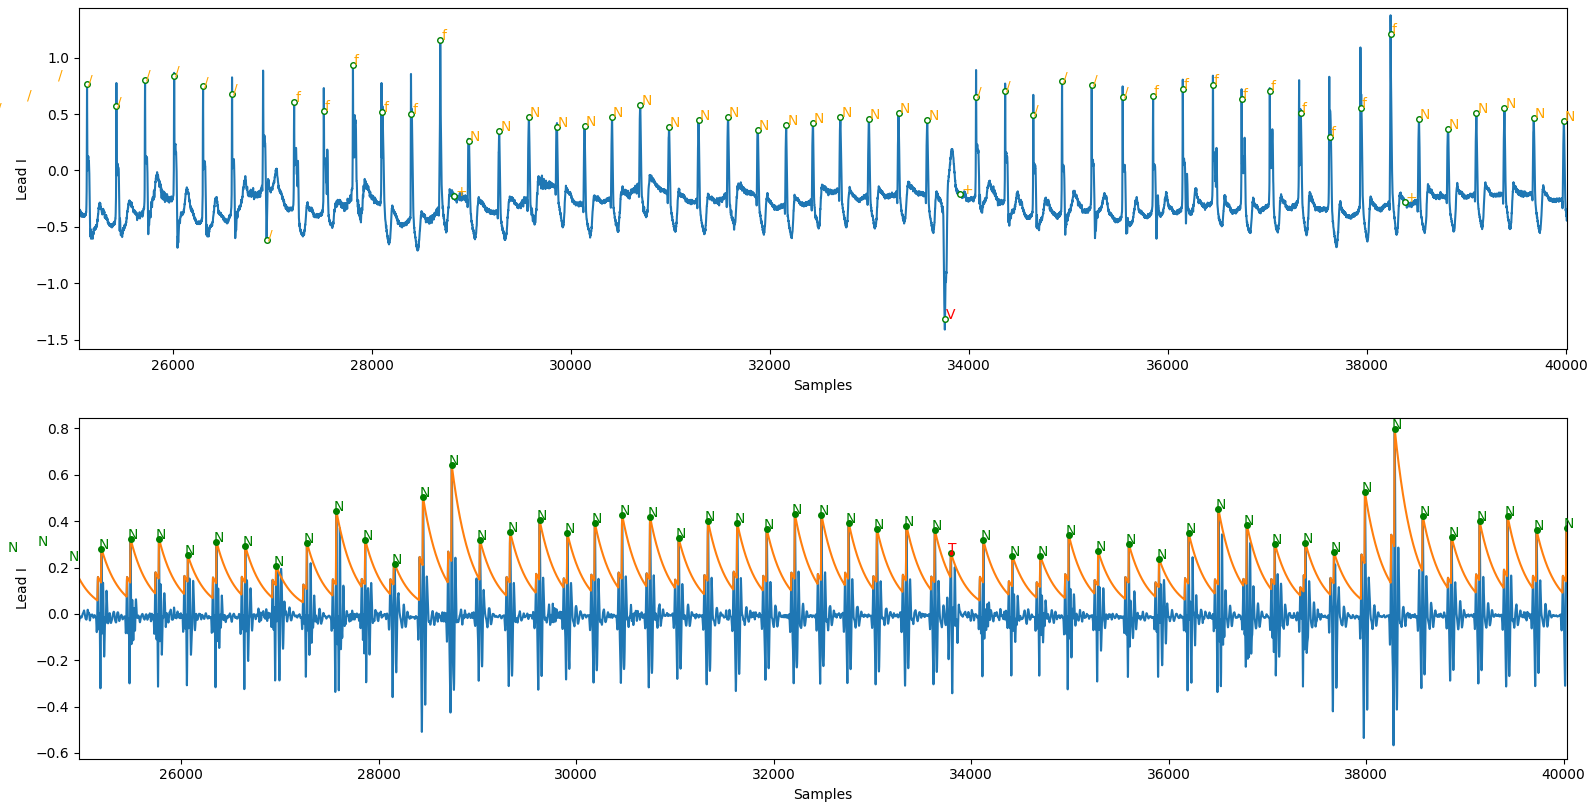
\includegraphics[width=0.99\textwidth]{./Images/img_introduccion/102filtrado_y_sin_filtrar.png}
	\caption{Ejemplo de electrocardiograma original y filtrado de paciente 102}
	\label{fig:102filtradoysinfiltrar}
\end{figure}

\section{Datos de referencia}
Los datos de referencia para probar el algoritmo han sido obtenidos de un estudio realizado en el Instituto de Tecnología de Massachusetts (MIT) \cite{MIT} en el que se han realizado pruebas de media hora a varios pacientes con edades diversas y algunos de ellos llevaban implantado un marcapasos.

Los datos consisten en electrocardiogramas que previamente han sido analizados por cardiólogos y cuyas anotaciones indican cuando un paciente ha padecido una arritmia, cuando el ritmo es normal y cuando se ha producido un fallo en la lectura de la señal, como se puede ver en la \cref{fig:Paciente_pruebas_MIT}. También se muestra información menos relevante para nuestro 
estudio como cuando se ha producido un error en la lectura de la señal y la activación del marcapasos\footnote{\textbf{Marcapasos}: Dispositivo que se implanta en el corazón que actúa cuando el corazón no bombea la sangre lo suficientemente fuerte, es decir que el pico QRS no es tan prominente
y se necesita la ayuda de dicho dispositivo para proporcionar el impulso eléctrico necesario}.

\begin{figure}[h]
	\centering
	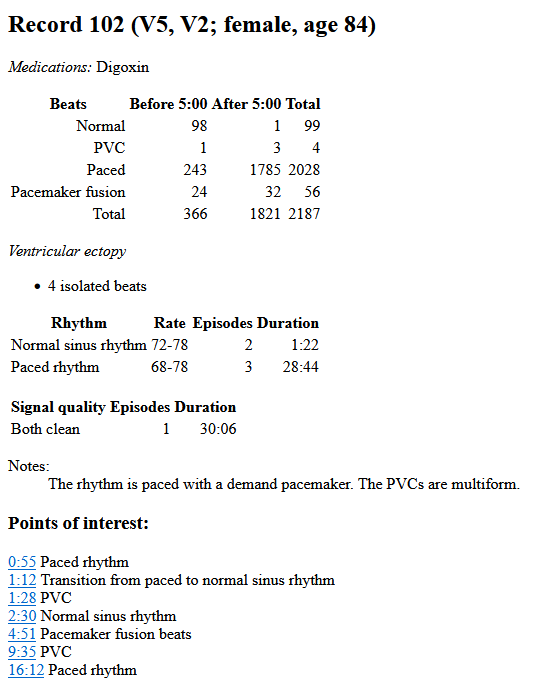
\includegraphics[width=0.6\textwidth]{./Images/img_introduccion/Paciente_pruebas_MIT.png}
	\caption{Ejemplo con paciente 102 \cite{mitdb}}
	\label{fig:Paciente_pruebas_MIT}
\end{figure}

\section{Utilización de las FPGAs}
Este algoritmo ha sido pensado para ejecutarse en un dispositivo pequeño, poco pesado y portable, es por ello que es conveniente ejecutarlo en una FPGA \cite{mdpi_sensors_2014}. Esto de debe a que hay FPGAs pequeñas que tienen el  \textit{hardware}  suficiente para poder llegar a ejecutar este algoritmo, además el consumo producido por una FPGA al ejecutar este algoritmo es bastante bajo como se comprobará posteriormente.

Para este proyecto se usó la FPGA Artix-7 \cite{xilinx_artix7} en la placa Basys3 para probar el funcionamiento del algoritmo. Sin embargo, para las pruebas, debido a la cantidad de valores de prueba sacados de la base de datos por cada paciente, se ha considerado utilizar otra FPGA cuyo  \textit{hardware}  pueda soportar dicha cantidad de datos.


\section{Objetivos del proyecto}

El objetivo principal del proyecto es crear un algoritmo basado en el estudio de caracterización de señales usando polinomios de Hermite \cite{desai2021low} que detecte arritmias en los pacientes y que dicho algoritmo sea capaz de ejecutarse en un dispositivo portátil, que tenga un bajo consumo y que funcione en tiempo real. Para lograr el objetivo principal es necesario alcanzar una serie de objetivos que son los siguientes:

\begin{enumerate}
    \item Averiguar qué son las arritmias, cómo se producen, qué arritmias podría detectar el programa y qué patrón siguen la mayoría de ellas.
    \item La creación de un algoritmo en software que sea capaz de leer y filtrar la señal original de los pacientes de la base de datos, la realización de un algoritmo que se encargue de detectar los picos donde se produce la contracción ventricular según aparecen en la señal filtrada y, por último, la creación de un algoritmo encargado de detectar las arritmias según el patrón hallado en el objetivo anterior.
    \item La replicación del programa en \textit{hardware} según el prototipo creado anteriormente en software. Utilizando el \textit{hardware} necesario para que el algoritmo funcione en una FPGA y el  \textit{hardware}  necesario para poder hacer pruebas en simulación y sobre la placa.
    \item La observación de los resultados experimentales de la cantidad de recursos \textit{hardware} empleados, el consumo utilizado por el algoritmo y el tiempo que tarda en llevarse a cabo adecuándose a la llegada de la señal del paciente. Dichos resultados experimentales deberían tener coherencia con lo que se buscaba en el objetivo principal.
\end{enumerate}


\section{Plan de trabajo}
\begin{enumerate}
	\item Investigación y fundamentación teórica:
	
	\begin{enumerate}
		\item Revisión del libro \cite{velez} y consulta con un médico especialista en primeros auxilios para comprender qué son las arritmias y cómo se producen.
	
		\item Utilizar la información obtenida para establecer la base médica del proyecto.
	\end{enumerate}

	\item Obtención y preparación de datos:
	\begin{enumerate}
		\item Localizar y descargar la base de datos del proyecto utilizada en el estudio de caracterización de señales usando polinomios de Hermite \cite{desai2021low}.

		\item Representar las señales en Python y realizar el filtrado según lo descrito en el estudio mencionado.
	\end{enumerate}
	\item Desarrollo de Algoritmos:
	\begin{enumerate}
		\item Implementar el algoritmo de detección de picos QRS y el algoritmo de detección de arritmias.

		\item Realizar pruebas y ajustes en los algoritmos para obtener resultados satisfactorios.
	\end{enumerate}
	
	\item Implementación en  \textit{hardware} : 
	\begin{enumerate}
		\item Diseñar los módulos principales para cada parte del algoritmo: detección de picos, detección de arritmias, filtrado y un módulo principal.

		\item Crear módulos adicionales para realizar simulaciones en Vivado y verificar el funcionamiento del programa.
		\item Desarrollar un \textit{testbench} para generar la frecuencia de reloj y las señales necesarias para simular el sistema.
	\end{enumerate}

	\item Análisis de resultados experimentales:
	\begin{enumerate}
		\item Evaluar los resultados obtenidos de los análisis realizados en Vivado.

		\item Extraer conclusiones relevantes en función de los objetivos del proyecto.
	\end{enumerate}
\end{enumerate}

\section{Análisis y optimización del algoritmo}
El algoritmo se centra en tres funciones principales:
\begin{enumerate}
\item Filtrado de la señal original: Se utiliza el filtrado FIR\cite{FIR}, lo que hace que la señal sea más fácil de procesar para encontrar los picos QRS. Esto se realiza multiplicando los valores de la señal original por los coeficientes de filtrado almacenados en una memoria.
\item Detección de picos sobre la señal filtrada: Se analiza cada valor de la señal filtrada y si dicho valor es mayor que sus anteriores, se considera un posible pico. Si después de 72 valores se mantiene como el valor más alto, entonces ese valor se considera un pico QRS. Adicionalmente, se establece un \textit{cutoff} dinámico en el que, si los picos de la señal no superan ese valor, no se tienen en cuenta.
\item Detección de arritmias comparando la posición de los picos: Una vez obtenidos los picos QRS, se calcula la distancia del pico actual con el pico anterior y, dependiendo de las distancias anteriores, se determina si hay una arritmia.
\end{enumerate}

\section{Implementación en la FPGA}
Para implementar el código en la FPGA se implementarán varios módulos que por lo general, tratan de replicar las funcionalidades que realiza el algoritmo de software y se convertirán en la parte más importante de dicho programa.  

Los módulos principales son.

	\begin{enumerate}
		\item Módulo de filtrado: Se guardan los coeficientes del filtrado en un módulo de memoria ROM y los valores de la señal original en una memoria RAM posteriormente, se multiplica cada muestra por su correspondiente coeficiente y se acumula el resultado. Una vez terminado el proceso de multiplicación y acumulación, el valor calculado se transmite al siguiente módulo principal.
		\item Módulo de detección de picos sobre la señal filtrada: Se implementa una máquina de estados que analiza cada valor de la señal filtrada y calcula si es un posible pico, o un pico QRS. Como los valores de la señal son números reales, se implementan varios módulos para poder operar con los valores de la señal en punto flotante. 
		\item Módulo de detección de arritmias: Se implementa una máquina de estados con el que recibiendo un pico QRS como entrada, sea capaz de almacenar las distancias más recientes, determinar según la diferencia de estas distancias, si se ha producido una arritmia y mostrar como salida un flag indicándolo.
	\end{enumerate}
	
	Además de estos módulos se debe crear un módulo que los encapsule y un \textit{testbench} para probar el funcionamiento del programa con las señales de la base de datos \cite{desai2021low}.

\section{Organización de la memoria}
En el capítulo 2 se verá cómo se ha realizado el prototipado del algoritmo en software. En la sección 2.1 se muestra el transcurso del algoritmo. En la sección 2.2, se indicarán las librerías usadas para la recopilación de datos. En la sección 2.3, se explicará el tipo de filtrado que se ha usado para la señal original. En la sección 2.4, se expondrá el algoritmo de detección de picos QRS y las metodologías seguidas. En la sección 2.5, se explicará el algoritmo de detección de arritmias y en la sección 2.6, el algoritmo para probar el prototipo y obtener estadísticas de las pruebas realizadas.

En el capítulo 3, se hablará de los distintos módulos creados para la implementación  \textit{hardware}. En la sección 1, se especificarán los módulos para las operaciones en punto flotante y las memorias utilizadas. De la sección 2 a la 4, se explicará el funcionamiento del módulo de filtrado de la señal, el módulo de detección de picos y el módulo de detección de arritmias. En la sección 5, se tratará la creación del módulo principal y el \textit{testbench} utilizado.

En el capítulo 4, se mostrarán los resultados experimentales obtenidos, como la FPGA utilizada, el análisis de utilización de  \textit{hardware}, el análisis de  \textit{timing} y el consumo.

Finalmente, en el capítulo 5, se dará una conclusión sobre la realización de este proyecto y se sugerirán trabajos futuros por si se desea ampliar el proyecto.
